% \documentclass[11pt]{report}
% \usepackage[left=1cm, right=1cm, top=2cm]{geometry}
\documentclass[headsepline,footsepline,oneside,fontsize=11pt,paper=a4,listof=totoc,bibliography=totoc,BCOR=12mm,DIV=13]{scrbook} % one-sided

\usepackage{ayad}
\usepackage[utf8]{inputenc}

\usepackage{settings}
% TODO: change thesis information
\newcommand*{\getUniversity}{Technische Universität München}
\newcommand*{\getFaculty}{Department of Informatics}
\newcommand*{\getTitle}{Uncertainty estimation in neural times series modelling}
\newcommand*{\getTitleGer}{Titel der Abschlussarbeit}
\newcommand*{\getAuthor}{Ahmed Ayyad}
\newcommand*{\getDoctype}{Master's Thesis in Informatics}
\newcommand*{\getSupervisor}{Professor Vasileios Belagiannis}
\newcommand*{\getAdvisor}{Doctor Shadi Albarqouni}
\newcommand*{\getSubmissionDate}{15th January 2020}
\newcommand*{\getSubmissionLocation}{Munich}



\begin{document}

\pagenumbering{alph}
\begin{titlepage}
  % HACK for two-sided documents: ignore binding correction for cover page.
  % Adapted from Markus Kohm's KOMA-Script titlepage=firstiscover handling.
  % See http://mirrors.ctan.org/macros/latex/contrib/koma-script/scrkernel-title.dtx,
  % \maketitle macro.
  \oddsidemargin=\evensidemargin\relax
  \textwidth=\dimexpr\paperwidth-2\evensidemargin-2in\relax
  \hsize=\textwidth\relax

  \centering

  \IfFileExists{logos/tum.pdf}{%
    
\includegraphics[height=20mm]{logos/tum.pdf}
  }{%
    \vspace*{20mm}
  }

  \vspace{5mm}
  {\huge\MakeUppercase{\getFaculty{}}}\\

  \vspace{5mm}
  {\large\MakeUppercase{\getUniversity{}}}\\

  \vspace{20mm}
  {\Large \getDoctype{}}

  \vspace{15mm}
  \makeatletter
  \ifthenelse{\pdf@strcmp{\languagename}{english}=0}
  {\huge\bfseries \getTitle{}}
  {\huge\bfseries \getTitleGer{}}
  \makeatother

  \vspace{15mm}
  {\LARGE \getAuthor{}}

  \IfFileExists{logos/faculty.png}{%
    \vfill{}
    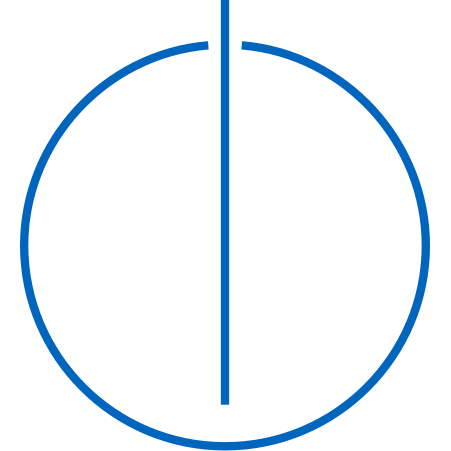
\includegraphics[height=20mm]{logos/faculty.png}
  }{}
\end{titlepage}




\frontmatter{}

\begin{titlepage}
  \centering

  \IfFileExists{logos/tum.pdf}{%
    
\includegraphics[height=20mm]{logos/tum.pdf}
  }{%
    \vspace*{20mm}
  }

  \vspace{5mm}
  {\huge\MakeUppercase{\getFaculty{}}}\\

  \vspace{5mm}
  {\large\MakeUppercase{\getUniversity{}}}\\

  \vspace{20mm}
  {\Large \getDoctype{}}

  \makeatletter
  \vspace{15mm}
  \ifthenelse{\pdf@strcmp{\languagename}{english}=0}
  {
  {\huge\bfseries \getTitle{}}

  \vspace{10mm}
  {\huge\bfseries \foreignlanguage{ngerman}{\getTitleGer{}}}
  }
  {
  {\huge\bfseries \getTitleGer{}}

  \vspace{10mm}
  {\huge\bfseries \foreignlanguage{english}{\getTitle{}}}
  }
  \makeatother

  \vspace{15mm}
  \begin{tabular}{l l}
    Author:          & \getAuthor{} \\
    Supervisor:      & \getSupervisor{} \\
    Advisor:         & \getAdvisor{} \\
    Advisor:         & \getSecondAdvisor{} \\
    Submission Date: & \getSubmissionDate{} \\
  \end{tabular}

  \IfFileExists{logos/faculty.png}{%
    \vfill{}
    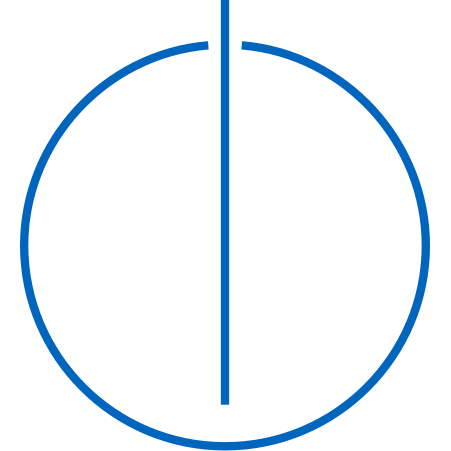
\includegraphics[height=20mm]{logos/faculty.png}
  }{}
\end{titlepage}


\cleardoublepage{}

\thispagestyle{empty}
\vspace*{0.8\textheight}
\noindent
I confirm that this \MakeLowercase{\getDoctype{}} is my own work and I have documented all sources and material used.

\vspace{15mm}
\noindent
\getSubmissionLocation{}, \getSubmissionDate{} \hspace{50mm} \getAuthor{}

\cleardoublepage{}

\

\addcontentsline{toc}{chapter}{Acknowledgments}

\thispagestyle{empty}

\vspace*{20mm}

\begin{center}
\usekomafont{section} Acknowledgments
\end{center}

\vspace{10mm}

%TODO: Acknowledgments
work in progress


\cleardoublepage{}

 

\chapter{Abstract}

%TODO: Abstract

The advancement of Machine Learning (ML) capabilities is making its deployment to complex real world problems appealing. In the automotive industry ML can be beneficial in a wide range of tasks, from providing cheaper or more accurate sensors, to autonomous control of vehicles. 
This thesis is focused on a key issue for the real world reliability of ML models: \textbf{Uncertainty estimation}.

The goal is to design models which can return an uncertainty signal along with their predictions. The crucial requirement being that when model errors are high the uncertainty should also be high.
% The ultimate goal of this line of research would be models that guarantee accurate predictions whenever their uncertainty estimates are low. For now, we present a model where we show a strong correlation between errors and uncertainties. Uncertainty estimates are important, because acting on incorrect predictions can have fatal consequences.
We find that out-out-distribution(OOD) inputs are a major source of errors for our models. We formalize the problem of estimating uncertainties when OOD inputs are present. We show that model predictions are only reliable when the input is \emph{similar} to what the model has seen during training, even for ensembles or standard Bayesian models.  

Based on this analysis, we introduce Compression Recurrent Neural Networks(C-RNN), an approach to learn time series predictors with robust uncertainty estimates. Our model is based on a principled and flexible approach to modelling the distribution of the training data, in order to deal with OOD inputs. 
We preform in-depth experiments, studying the relationship between OOD inputs, model errors and model uncertainties, for our C-RNN model and MC dropout~\citep{gal2016dropout}. Our results show that uncertainty estimates from C-RNN are consistently more informative that MC dropout's. In our experiments on the Revs vehicle dynamics database, C-RNN manages to effectively eliminate OOD inputs with an Area under the ROC curve of 0.97, and manages to capture errors with a correlation of 0.85 between the errors and the uncertainty. 



% Out-of-distribution(OOD) detection, is becoming a crucial problem for modern machine learning. As models are being deployed in critical systems, we need a robust estimate of the model's certainty over its predictions. We argue that reliable uncertainty estimation must take into account the \emph{similarity} between the current input and the training distribution. Accordingly, we present a recurrent compression model which can detect low-probability inputs. 


\microtypesetup{protrusion=false}
\tableofcontents{}
\microtypesetup{protrusion=true}

% \section*{Notation}

% \ahmed{For now this section is just to help me keep things consistent, plan is to clean or remove it in final version}

% \begin{itemize}

% \item Bold capital letters $\mathbf{A}$ represent matrices

% \item Bold lower case letters $\mathbf{v}$ represent vectors

% \item Lower case greek symbol ($\theta$) represent model parameters

% \item The calligraphic $\mathcal{X}$ represents the input space

% \item The calligraphic $\mathcal{Y}$ represents the target space

% \item \pdf{.} is the probability density function

% \item \pdf[t]{.} is the pdf under some distribution $t$ 

% \item \pdf{.|\theta} is the pdf as modeled by parameters $\theta$ 

% \item $\mathbb{E}_{q}[f(.)]$ represents an expectation of function $f$ under $q$

% % \item Lower case letters $(x, y)$ represent random variables 

% \item The upper case letters $X, Y$ represent matrices of the training and target samples

% \item Predictive distribution denotes predictions that come in the form of probability distribution rather than a point prediction

% \end{itemize}

\mainmatter{}

\chapter{Introduction}
\subfile{Intro/Intro.tex}

\chapter{Background}
\label{ch:background}
\subfile{Background/Backgound.tex}


\chapter{Approach}
\label{ch:approach}
\subfile{Approach/Approach.tex}


\chapter{Experiments}
\label{ch:experiments}
\subfile{Experiments/Experiments.tex}

\chapter{Related work}
\subfile{RelatedWork/RelatedWork.tex}


\chapter{Conclusion}
\subfile{Conclusion/Conclusion.tex}



\newpage
\appendix
\chapter{Appendix}


\chapter{General Addenda}

If there are several additions you want to add, but they do not fit into the thesis itself, they belong here.

\section{Detailed Addition}

...




\end{document}
